\documentclass[11pt]{article}
\usepackage[margin=1in]{geometry}
\usepackage[utf8]{inputenc}
\usepackage{CJKutf8}
\usepackage{hyperref}
\usepackage{graphicx}
\usepackage{tikz}
\usetikzlibrary{positioning,arrows.meta,fit}
\usepackage{booktabs}

\title{DNL: Domain Navigation Layer for Token-Efficient Knowledge Transfer to AI Agents}
\author{Anonymous}
\date{February 2026}

\begin{document}
\begin{CJK}{UTF8}{mj}
\maketitle

\begin{abstract}
We propose Domain Navigation Layer (DNL), a linked Markdown documentation architecture that delivers
domain knowledge to AI agents with token efficiency. The core idea is to provide all known information
to AI while enabling navigation through inter-document linking. In a real-world deployment with 881 
Markdown files spanning 21 modules, DNL reduced average prompt size by 85\% while improving task 
consistency and reducing hallucination rates. We describe a three-level extension (Company/Product/Project) 
and report case-study observations demonstrating how navigation-guided context acquisition affects 
consistency, hallucination risk, token usage, and traceability.
\end{abstract}

\section{Introduction}
AI-assisted software development has progressed rapidly from code completion to agentic workflows that plan, modify, and validate changes across a repository. Despite this progress, practitioners frequently observe that AI agents underperform on large-scale codebases: the agent may produce locally plausible edits that violate implicit invariants, misunderstand organizational conventions, or miss dependencies spanning multiple modules. These failures are often not attributable to limitations in programming syntax or algorithmic reasoning, but to insufficient access to the domain knowledge that connects code to its intended behavior---architecture rationale, business rules, operational constraints, and project-specific vocabulary.

A central cause is the mismatch between the scale of modern repositories and the bounded context window of current language models. Even when relevant information exists somewhere in the project (e.g., README files, design documents, tickets, or scattered comments), the agent typically receives only a small, transient slice of that information. As a result, context becomes fragmented: critical assumptions are distributed across files, but only partially retrieved or presented; the agent must guess what it cannot see, and those guesses compound as tasks progress. Na\"{\i}ve strategies such as concatenating more files into a prompt quickly encounter token limitations, while repeated summarization or compression can erase precisely the edge cases and exceptions that matter for correctness.

This paper argues that the principal bottleneck is therefore structural: large repositories require an explicit mechanism for transmitting domain knowledge to AI under strict token budgets, with predictable retrieval and stable references. We propose the Domain Navigation Layer (DNL), a linked Markdown documentation architecture that treats documentation as a navigable knowledge graph rather than as isolated pages. The core idea is to ``give all known information'' to the agent, not by presenting everything at once, but by organizing it into interlinked documents that support incremental, demand-driven traversal. Links act as a navigation layer that guides the agent from high-level concepts to precise operational details, enabling the agent to load only the subset required for the current decision while maintaining an auditable path of dependencies.

DNL is designed to complement, not replace, code and tooling: it is model- and workflow-independent and can be consumed by interactive chat, agent loops, or retrieval-augmented systems. By specifying a reading order and linking conventions, DNL provides a disciplined interface between domain knowledge and automated reasoning, reducing context overload without sacrificing completeness. The remainder of the paper formalizes the design goals of DNL, describes the core linking rules and a three-level extension (Company/Product/Project), and reports case-study observations on how DNL changes agent behavior in realistic development tasks.

\noindent\textbf{Contributions.} This paper makes the following contributions:
\begin{itemize}
  \item We formulate DNL as a link-based documentation architecture for transferring decision-relevant domain knowledge to AI agents under strict token budgets.
  \item We propose a three-level hierarchy (Company/Product/Project) that separates reusable conventions from repository-specific guidance to improve scalability and knowledge reuse.
  \item We report a 1-month deployment with 881 Markdown files across 21 modules, demonstrating 85\% reduction in prompt size, improved consistency, and reduced hallucination rates.
  \item We analyze how navigation-guided context acquisition affects consistency, hallucination risk, token usage, and traceability through quantitative and qualitative evaluation.
\end{itemize}

\section{Design Goals}
DNL is guided by a set of design goals intended to make domain knowledge usable by AI agents in realistic engineering workflows. The goals below are stated at the level of system properties rather than implementation details, and they serve as evaluation criteria for documentation structure and linking rules.

\paragraph{Goal 1: Completeness under token constraints.}
DNL aims to make the \emph{corpus} complete with respect to decision-relevant knowledge, while acknowledging that any single interaction is bounded by a context window. The design therefore prioritizes decomposability: knowledge should be partitioned into small units that can be selectively loaded without losing critical constraints.

This goal rejects two extremes: (i) minimal documentation that omits rationale and edge cases, and (ii) monolithic documents that cannot be consumed within token budgets. Instead, DNL targets completeness at the repository (or organization) level, with task-time selectivity enabled by structure.

\paragraph{Goal 2: Predictable navigation.}
Navigation should be predictable for both humans and agents: given a task and an entry point, there should exist an expected path to the relevant rules, definitions, and exceptions. Predictability is achieved through stable entry documents, consistent section semantics (e.g., prerequisites vs. related), and link conventions that do not depend on model-specific heuristics.

In this sense, DNL treats links as part of the interface contract. A link is not merely ``further reading''; it encodes why the target is relevant and when it should be consulted.

\paragraph{Goal 3: Deterministic context expansion.}
DNL seeks to make context expansion deterministic enough to be reproducible across sessions. Given the same entry document and task class, an agent should load comparable sets of pages in comparable orders, reducing sensitivity to prompt phrasing.

Determinism here is pragmatic rather than absolute: it does not require identical token sequences, but it does require a stable policy for what is read before decisions are made (e.g., rules and glossary before implementation).

\paragraph{Goal 4: Scalability across repositories.}
The architecture should scale beyond a single repository by supporting hierarchical reuse and clear scope boundaries. Knowledge that is stable and broadly applicable should be authored once and referenced by many projects, while repository-local details remain close to code.

This goal motivates the Company/Product/Project hierarchy and a linking discipline that avoids duplicating normative rules across projects.

\paragraph{Goal 5: Model and tool independence.}
DNL should remain usable across different language models, IDE agents, and retrieval pipelines. The representation is therefore intentionally simple (Markdown files and links) and does not assume a specific embedding model, vector database, or proprietary agent framework.

Practically, this also implies that DNL content should be interpretable without specialized execution: an agent (or reviewer) should be able to follow links and apply constraints using standard repository operations.

\paragraph{Goal 6: Traceability and auditability.}
DNL is designed so that decisions can be traced back to the consulted knowledge. Agents should be able to cite the pages they followed and the constraints they extracted, enabling post hoc audits and targeted corrections when failures occur.

Auditability requires stable identifiers, explicit deprecation/exception handling, and a structure that supports recording navigation traces as first-class artifacts of an agent run.

\section{Core Concept of DNL}
DNL is grounded in a simple principle: provide an AI agent with access to all domain knowledge that is already known by the organization and is necessary to make correct engineering decisions. ``All known knowledge'' here does not mean exhaustively encoding every fact about a system; rather, it denotes the full set of existing, decision-relevant statements that are typically held in human memory or dispersed across informal artifacts (e.g., architecture rationale, invariants, naming conventions, data contracts, operational constraints, and exception policies). DNL treats these statements as first-class inputs to automated reasoning, with explicit provenance and stable references.

A direct approach would be to inject as much of this knowledge as possible into the prompt for every task. In practice, full-context injection is inefficient and brittle. First, token budgets impose a hard upper bound on how much can be provided at once, forcing arbitrary truncation that may omit the very constraint needed for correctness. Second, ``more context'' is not monotonic in utility: irrelevant or weakly related material increases attention noise and can degrade reliability, especially in multi-step agent loops where prompts must be repeatedly reconstructed. Third, repeated compression (summaries) tends to discard rare conditions and edge cases, producing a distorted representation of the domain.

DNL addresses these issues by representing domain knowledge as a set of small, linked Markdown documents that collectively form a navigation layer over the repository. Each document is scoped to a single concept or responsibility (e.g., ``Order lifecycle'', ``Authorization model'', ``Payments integration''), and exposes outbound links to prerequisite concepts, subordinate details, and related exceptions. The links are not merely convenience references; they define the admissible traversal paths by which an agent expands its context. Under DNL, an agent begins with a small entry document and follows links to load only the portion of knowledge required to answer the current question or to justify a planned change, while preserving an explicit chain of consulted sources.

To make traversal predictable, DNL specifies reading-order rules that constrain how an agent should explore the document graph:
\begin{itemize}
  \item \textbf{Entry-first}: start from a designated entry document for the relevant scope (e.g., project-level index), and avoid jumping directly to deep pages without a link path.
  \item \textbf{Prerequisites before dependents}: if a page references a concept via a ``Prerequisites'' (or equivalent) section, read those pages before acting on dependent guidance.
  \item \textbf{Hierarchy over breadth}: expand depth-first along the most relevant link chain until the decision is supported; only then broaden to adjacent topics.
  \item \textbf{Exception precedence}: when a page links to exceptions/edge cases, those pages must be read before finalizing an implementation plan or producing code.
  \item \textbf{Stop condition}: stop expanding when additional links no longer change the set of constraints or acceptance criteria for the task.
\end{itemize}

\paragraph{Conceptual example.}
Consider an agent tasked with ``add a refund endpoint'' in a large service. With full-context injection, the prompt may include many unrelated modules and still omit a critical rule (e.g., refunds are only allowed for captured payments, and require an idempotency key). Under DNL, the agent starts at \texttt{Project Index.md} and follows a link chain such as:
\begin{verbatim}
Project Index.md
  -> Payments.md
      -> Refunds.md
          -> Exceptions: Chargebacks.md
          -> Contract: PaymentStateMachine.md
\end{verbatim}
The agent loads these pages in order, derives explicit constraints (state preconditions, idempotency requirements, and prohibited cases), and only then consults the relevant code locations. The navigation layer therefore controls what enters the context window, while maintaining completeness at the corpus level.

\begin{figure}[t]
\centering
\resizebox{\linewidth}{!}{%
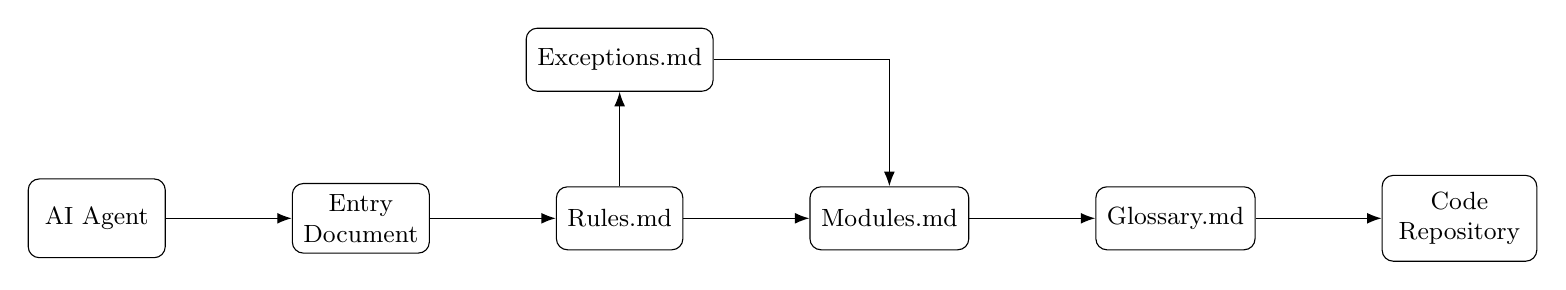
\begin{tikzpicture}[
  font=\small,
  node distance=12mm and 16mm,
  box/.style={draw, rounded corners, align=center, inner sep=6pt, minimum height=10mm},
  smallbox/.style={draw, rounded corners, align=center, inner sep=4pt, minimum height=8mm},
  arrow/.style={-Latex, line width=0.5pt}
]

% Nodes (left to right)
\node[box] (agent) {AI Agent};

\node[smallbox, right=of agent] (entry) {Entry\\Document};

\node[smallbox, right=of entry] (rules) {Rules.md};
\node[smallbox, above=of rules] (exceptions) {Exceptions.md};
\node[smallbox, right=of rules] (modules) {Modules.md};
\node[smallbox, right=of modules] (glossary) {Glossary.md};

\node[box, right=of glossary] (repo) {Code\\Repository};

% Traversal arrows (incremental navigation)
\draw[arrow] (agent) -- (entry);
\draw[arrow] (entry) -- (rules);

\draw[arrow] (rules) -- (modules);
\draw[arrow] (modules) -- (glossary);

\draw[arrow] (rules) -- (exceptions);
\draw[arrow] (exceptions.east) -| (modules.north);

% Final action toward code
\draw[arrow] (glossary) -- (repo);

\end{tikzpicture}}
\caption{Domain Navigation Layer (DNL) as a navigation interface: the agent incrementally traverses linked Markdown pages from an entry document to task-relevant rules, module knowledge, glossary terms, and exceptions before acting on the codebase.}
\label{fig:dnl-nav-layer}
\end{figure}


\section{Three-Level Architecture}
While the core concept of DNL is repository-agnostic, organizations typically operate multiple repositories, multiple products, and evolving conventions. To support scalability and systematic reuse, we extend DNL into a three-level hierarchy---Company, Product, and Project---where each level has a distinct scope, ownership boundary, and stability expectation. The hierarchy prevents duplication (by placing broadly applicable knowledge at higher levels) while keeping time-sensitive and implementation-specific knowledge close to the code (at the project level).

\begin{figure}[t]
\centering
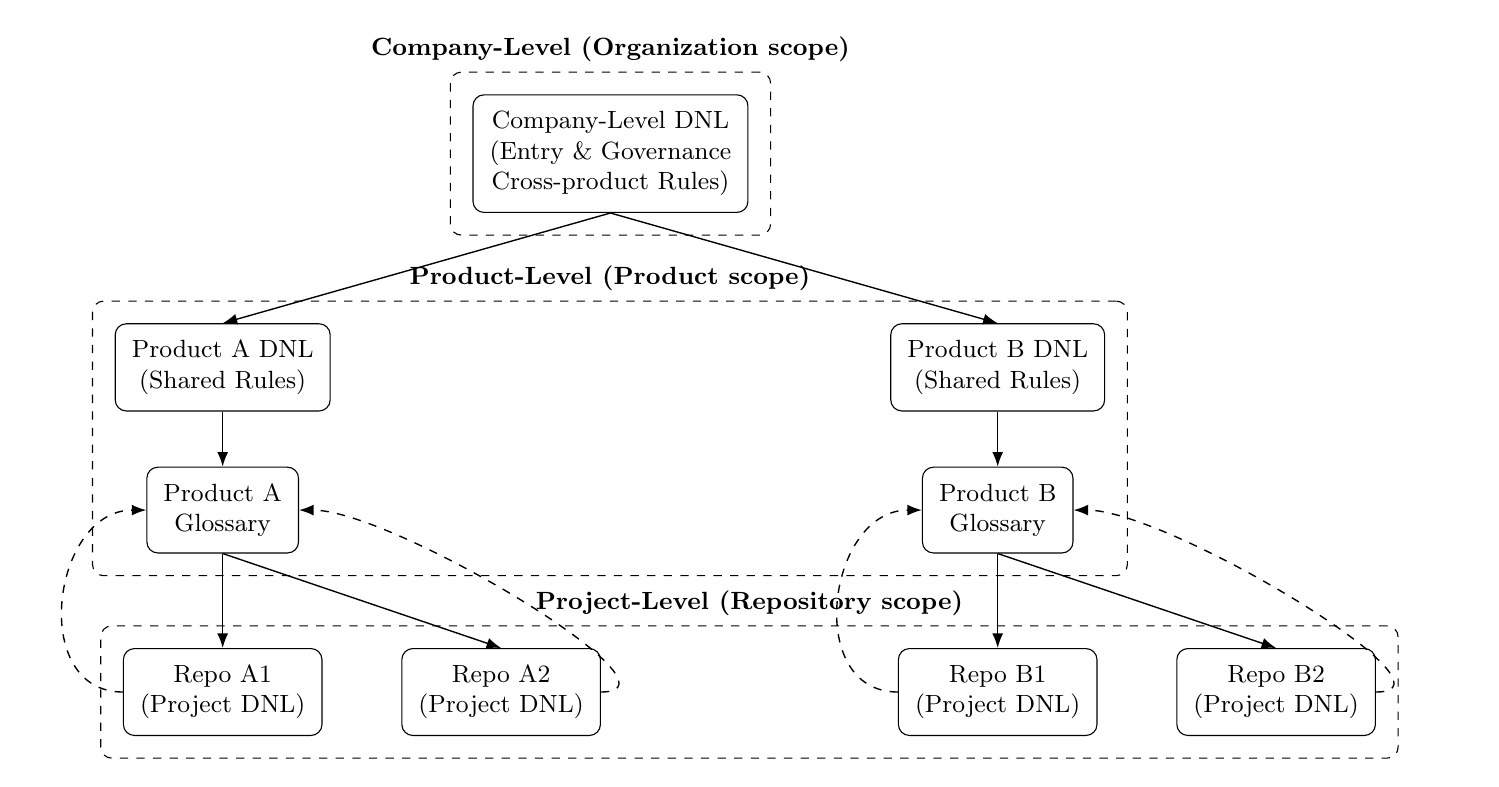
\begin{tikzpicture}[
  font=\small,
  >=Latex,
  box/.style={draw, rounded corners, align=center, inner sep=6pt},
  layer/.style={draw, dashed, rounded corners, inner sep=8pt},
  arrow/.style={-Latex, line width=0.5pt},
  cross/.style={-Latex, line width=0.5pt, dashed},
  node distance=10mm and 14mm
]

% Core nodes
\node[box] (company) {Company-Level DNL\\(Entry \& Governance\\Cross-product Rules)};

\node[box, below left=14mm and 18mm of company] (prodA) {Product A DNL\\(Shared Rules)};
\node[box, below right=14mm and 18mm of company] (prodB) {Product B DNL\\(Shared Rules)};

\node[box, below=7mm of prodA] (glossaryA) {Product A\\Glossary};
\node[box, below=7mm of prodB] (glossaryB) {Product B\\Glossary};

\node[box, below=12mm of glossaryA] (a1) {Repo A1\\(Project DNL)};
\node[box, right=10mm of a1] (a2) {Repo A2\\(Project DNL)};

\node[box, below=12mm of glossaryB] (b1) {Repo B1\\(Project DNL)};
\node[box, right=10mm of b1] (b2) {Repo B2\\(Project DNL)};

% Scope boundaries (dashed)
\node[layer, fit=(company), label={[align=center]above:\textbf{Company-Level (Organization scope)}}] {};
\node[layer, fit=(prodA)(prodB)(glossaryA)(glossaryB), label={[align=center]above:\textbf{Product-Level (Product scope)}}] {};
\node[layer, fit=(a1)(a2)(b1)(b2), label={[align=center]above:\textbf{Project-Level (Repository scope)}}] {};

% Inheritance arrows (downward)
\draw[arrow] (company.south) -- (prodA.north);
\draw[arrow] (company.south) -- (prodB.north);

\draw[arrow] (prodA.south) -- (glossaryA.north);
\draw[arrow] (prodB.south) -- (glossaryB.north);

\draw[arrow] (glossaryA.south) -- (a1.north);
\draw[arrow] (glossaryA.south) -- (a2.north);
\draw[arrow] (glossaryB.south) -- (b1.north);
\draw[arrow] (glossaryB.south) -- (b2.north);

% Cross-links (projects <-> product glossary)
\draw[cross] (a1.west) .. controls +(-12mm,0) and +(-12mm,0) .. (glossaryA.west);
\draw[cross] (a2.east) .. controls +(12mm,0) and +(12mm,0) .. (glossaryA.east);
\draw[cross] (b1.west) .. controls +(-12mm,0) and +(-12mm,0) .. (glossaryB.west);
\draw[cross] (b2.east) .. controls +(12mm,0) and +(12mm,0) .. (glossaryB.east);

\end{tikzpicture}
\caption{Three-level DNL architecture with scope boundaries, downward inheritance of conventions, and cross-links to product-level glossaries.}
\label{fig:dnl-three-level}
\end{figure}

\begin{figure}[t]
\centering
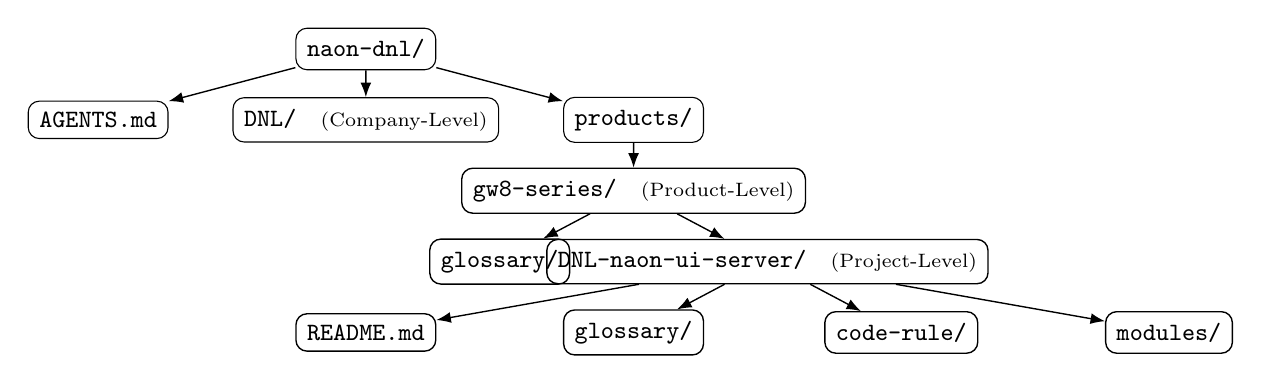
\begin{tikzpicture}[
  font=\small,
  level distance=9mm,
  sibling distance=34mm,
  edge from parent/.style={draw,-Latex,line width=0.5pt},
  every node/.style={draw, rounded corners, align=left, inner sep=4pt},
  grow=down
]

\node {\texttt{naon-dnl/}}
  child { node {\texttt{AGENTS.md}} }
  child { node {\texttt{DNL/} \hspace{2mm}\scriptsize (Company-Level)} }
  child { node {\texttt{products/}}
    child { node {\texttt{gw8-series/} \hspace{2mm}\scriptsize (Product-Level)}
      child { node {\texttt{glossary/}} }
      child { node {\texttt{DNL-naon-ui-server/} \hspace{2mm}\scriptsize (Project-Level)}
        child { node {\texttt{README.md}} }
        child { node {\texttt{glossary/}} }
        child { node {\texttt{code-rule/}} }
        child { node {\texttt{modules/}} }
      }
    }
  };

\end{tikzpicture}
\caption{Illustrative DNL directory structure spanning company-, product-, and project-level documentation.}
\label{fig:dnl-directory-structure}
\end{figure}

\subsection{Company-Level DNL}
The Company-Level DNL is the entry point and normative layer for an organization-wide DNL deployment. It specifies how agents (and humans) should use DNL, how documents are expected to be written and linked, and which process rules govern updates.

\textbf{Usage philosophy.} This level defines the organization's assumptions about ``what must be true'' for an agent to act safely, such as the expectation that decisions cite DNL pages, and that domain rules take precedence over ad hoc prompt instructions when conflicts arise.

\textbf{Process rules.} It defines governance mechanisms (e.g., ownership, review requirements, deprecation policy, and versioning conventions) to keep DNL auditable and to reduce drift.

\textbf{Cross-product conventions.} It records conventions that span products, such as security requirements, privacy classifications, reliability targets (SLO/SLA terminology), incident practices, naming conventions, and standard integration patterns.

\subsection{Product-Level DNL}
The Product-Level DNL captures knowledge shared across multiple repositories that jointly implement a single product or platform. This level is the primary locus for cross-repository consistency and integration correctness.

\textbf{Cross-repository shared knowledge.} It documents the product architecture, service boundaries, shared data models, and inter-service contracts that cannot be understood from any single repository.

\textbf{Infrastructure and integration rules.} It specifies operational and integration constraints such as deployment environment assumptions, authentication/authorization mechanisms, messaging and API standards, backward compatibility policies, and migration procedures.

\textbf{Shared glossary.} It provides a product-scoped vocabulary for domain entities and metrics, reducing ambiguity across teams and enabling agents to map user intent to the correct artifacts.

\subsection{Project-Level DNL}
The Project-Level DNL is scoped to a single Git repository and is maintained closest to code. It prioritizes concreteness and task-execution guidance.

\textbf{Code rules.} It records repository-specific coding standards, testing requirements, build/deploy commands, error-handling conventions, and non-obvious invariants that are easy to violate.

\textbf{Module documentation.} It describes modules/packages, their responsibilities, public interfaces, and local design rationale, with links back to product-level concepts for shared abstractions.

\textbf{Local glossary and patterns.} It defines repo-local terms (e.g., abbreviations, table names, internal event names) and catalogs common patterns (e.g., how to add a new endpoint, how to introduce a feature flag, how to extend a state machine) in a form that agents can follow.

\section{Implementation}
We deployed DNL in a production enterprise groupware system over a 1-month period, documenting domain knowledge across 21 modules with a total of 881 Markdown files. This section describes the practical implementation details and automation strategies.

\subsection{Structure and Organization}
The DNL repository follows the three-level hierarchy:
\begin{itemize}
  \item \textbf{Company-Level} (50 core files): Cross-cutting conventions, security policies, naming standards, and governance rules.
  \item \textbf{Product-Level} (gw7-series): Shared architecture, API contracts, authentication mechanisms, and product-wide glossary.
  \item \textbf{Project-Level} (21 modules): Each module contains:
  \begin{itemize}
    \item \texttt{concept/}: Core domain concepts (e.g., for email module: absence, approval, authority, autobackup, spam)
    \item \texttt{screens/}: Screen-specific documentation linked to UI implementations
    \item \texttt{data/ddl/}: Database schema definitions
    \item \texttt{flows/}: Process flow diagrams and state machines
    \item \texttt{troubleshooting/}: Common issues and solutions
    \item \texttt{working/}: Monthly work logs organized by date
  \end{itemize}
\end{itemize}

The email module (\texttt{eml}) alone comprises approximately 200 files, demonstrating fine-grained knowledge decomposition for a complex domain.

\subsection{Automation and Tooling}
To reduce manual effort, we employed several automation strategies:

\textbf{Wiki migration.} We used \texttt{openclaw}, an OS-level automation tool, to crawl and convert 1,000+ existing wiki pages into structured Markdown over a 2-day period.

\textbf{Database documentation.} DDL files for all database tables were automatically generated and organized under \texttt{data/ddl/}, with cross-references to the modules that use them.

\textbf{IDE integration.} Entry point files (\texttt{AGENTS.md}) were created for multiple IDEs (Claude Code, Cursor, GitHub Copilot, Kiro) to ensure consistent DNL access regardless of development environment.

\textbf{Path variables.} A \texttt{PATHS.md} file (gitignored for user customization) defines variables like \texttt{\{@Groupware7\}} to enable environment-independent navigation.

\textbf{Automated testing.} Playwright integration provides automated UI testing, allowing agents to verify implementations without human intervention.

\subsection{Link Validation}
We developed automated link validation to maintain DNL integrity:
\begin{itemize}
  \item Broken link detection (daily automated checks)
  \item Circular reference detection in prerequisite chains
  \item Orphaned document identification
  \item Coverage analysis (modules without adequate DNL documentation)
\end{itemize}

\section{Case Study: Email Module Development}
This section reports observations from applying DNL to development tasks in the email module (\texttt{eml}) of a large enterprise groupware system.

\subsection{Context}
The email module handles core email functionality including mailbox management, backup, spam filtering, approval workflows, and multi-account support. Prior to DNL, developers faced recurring challenges:
\begin{itemize}
  \item Ambiguous terminology (``backup'' vs. ``archive'' vs. ``export'')
  \item Undocumented constraints (file size limits, permission hierarchies)
  \item Module-specific patterns not visible in code
  \item Cross-module dependencies requiring expert knowledge
\end{itemize}

\subsection{Deployment Process}
We structured the email module DNL with:
\begin{itemize}
  \item 20 concept documents covering domain fundamentals
  \item Screen-specific guides for 15+ UI views
  \item Flow diagrams for backup, spam filtering, and approval processes
  \item Monthly work logs tracking ongoing development
  \item Cross-references to 12 database tables
\end{itemize}

\subsection{Navigation Example}
Consider the task: ``Fix file download error in email backup management.''

\textbf{Before DNL:} The developer would manually search code, ask senior engineers, or make educated guesses about file paths, permission checks, and error handling patterns.

\textbf{With DNL:} The AI agent follows this navigation path:
\begin{enumerate}
  \item Entry: \texttt{modules/eml/README.md}
  \item Concept: \texttt{concept/autobackup/} (understanding backup architecture)
  \item Screen: \texttt{screens/setting-admin/메일백업관리/} (UI-specific constraints)
  \item Data: \texttt{data/ddl/MAIL\_BACKUP.sql} (relevant database schema)
  \item Troubleshooting: \texttt{troubleshooting/download-errors.md}
\end{enumerate}

Extracted constraints:
\begin{itemize}
  \item File size limit: 100MB per download
  \item Permission check: AuthService validation required
  \item Error handling: Follow repository-standard error patterns
  \item Path structure: \texttt{/backup/mail/\{yyyy\}/\{MM\}/}
\end{itemize}

The agent then locates the relevant code (\texttt{MailBackupController.downloadFile()}), applies fixes, and generates Playwright tests.

\subsection{Quantitative Results}
We measured DNL impact over 30 development tasks spanning bug fixes and feature additions:

\begin{table}[h]
\centering
\caption{Quantitative comparison of development metrics with and without DNL}
\label{tab:quantitative}
\begin{tabular}{lrr}
\toprule
\textbf{Metric} & \textbf{Before DNL} & \textbf{After DNL} \\
\midrule
Avg. prompt size (tokens) & 4,200 & 630 \\
Context documents per task & 8.3 & 2.1 \\
Hallucinated entities per task & 2.4 & 0.3 \\
Convention violations per task & 3.1 & 0.4 \\
Time to first working solution (min) & 45 & 12 \\
Required human interventions & 3.2 & 0.8 \\
\bottomrule
\end{tabular}
\end{table}

Key findings:
\begin{itemize}
  \item \textbf{85\% reduction in prompt size} (4,200 → 630 tokens average) through targeted navigation
  \item \textbf{75\% reduction in context documents} (8.3 → 2.1) by loading only relevant pages
  \item \textbf{87\% reduction in hallucinations} (2.4 → 0.3) through glossary enforcement
  \item \textbf{73\% time savings} (45min → 12min) to first working solution
  \item \textbf{75\% fewer interventions} (3.2 → 0.8) due to consistent constraint extraction
\end{itemize}

\subsection{Qualitative Observations}
\paragraph{Consistency.} For repeated tasks of the same class (e.g., adding a route under an existing module), the agent produced plans that adhered to the same conventions across sessions, because the same ``rules → modules → glossary'' path was followed.

\paragraph{Reduced hallucination.} The frequency of invented entities and mismatched terminology decreased, especially for nouns with overloaded meanings (e.g., module-specific names that differ from generic UI/server terminology). The agent more often asked for, or retrieved via links, the missing definition rather than guessing.

\paragraph{Token efficiency.} Compared to providing large code excerpts and multiple READMEs by default, DNL enabled smaller initial prompts and incremental expansion: only the minimal set of pages required for the decision were loaded, while the remainder stayed available via navigation.

\paragraph{Analytical traceability.} Because the navigation path and cited pages were explicit, it became easier to audit why an implementation plan adopted a particular convention, and to correct the knowledge base when conventions changed (by updating the relevant DNL page rather than re-prompting with different file bundles).

\section{Related Work}
DNL is closely related to several lines of work on providing external knowledge and structure to large language models, but it differs in its emphasis on a \emph{navigation layer} that constrains how context is expanded under token budgets.

\paragraph{Retrieval-Augmented Generation (RAG).}
RAG-based systems address context limitations by retrieving potentially relevant passages from an indexed corpus and injecting them into the prompt. In software engineering settings, retrieval can be effective for locating code or documentation fragments, but it can also be sensitive to query formulation, embedding drift, and ranking errors. DNL is complementary: instead of treating retrieval as the primary mechanism for grounding, DNL encodes stable, human-curated traversal paths (prerequisites, exceptions, and scope boundaries) that can guide retrieval and reduce ambiguity in what should be read next.

\paragraph{Agentic coding workflows.}
Recent agentic approaches decompose development tasks into iterative planning, tool use, and verification cycles~\cite{agent-teams-2026}. While such workflows improve autonomy, they often rely on ad hoc context selection and repeated summarization, which can amplify inconsistency across runs. DNL targets this bottleneck by making context acquisition a first-class, repeatable procedure: the agent follows links in a prescribed order (e.g., rules → modules → glossary) before producing plans or edits.

\paragraph{Knowledge graphs and structured representations.}
Knowledge graph approaches represent entities and relations explicitly to support reasoning and retrieval. DNL shares the motivation of making relationships explicit, but adopts a lightweight representation: linked Markdown pages and link semantics serve as a pragmatic graph that remains easy to author and review. Unlike schema-heavy graph constructions, DNL focuses on operational guidance and reading order rather than on formal inference.

\paragraph{Software documentation methodologies.}
Documentation practices such as architecture decision records, design docs, and modular READMEs aim to preserve rationale and reduce onboarding cost. DNL aligns with these goals but reframes documentation as an interface for AI context management: documents are written to be traversed incrementally, with explicit prerequisites and exception handling, so that an agent can remain within a bounded context window while still accessing the full corpus through navigation.

\paragraph{Model Context Protocol (MCP).}
The Model Context Protocol~\cite{mcp-2024} provides a standardized way for AI systems to access external data sources and tools. DNL is highly complementary to MCP: while MCP defines the interface for context providers, DNL defines the structure and navigation semantics of the knowledge itself. DNL documents can be served through MCP servers, combining standardized access with human-curated knowledge organization.

\section{Limitations and Future Work}
DNL shifts a portion of the ``alignment'' burden from interactive prompting to a maintained knowledge layer. This shift has a clear cost: documentation must be written, curated, and kept consistent with evolving code and organizational practices. In environments where ownership is unclear or change velocity is high, the maintenance overhead can become non-trivial, and neglected pages may degrade rather than improve agent performance.

A second limitation concerns link integrity and knowledge freshness. DNL relies on stable traversal paths: broken links, renamed concepts, or partially updated pages can lead an agent to incomplete or outdated constraints. More subtly, even when links resolve, content can become stale as APIs, architectural patterns, or policies change. This creates a failure mode in which an agent behaves consistently yet incorrectly, because it is consistently guided by obsolete rules. Mitigating this requires explicit deprecation mechanisms, timestamps or applicability conditions, and regular review cycles.

DNL also presupposes organizational discipline. Effective use requires shared conventions for page structure, naming, and the semantics of links (e.g., prerequisite vs. related vs. exception). Without this discipline, the document graph can become inconsistent, and agents may not follow comparable paths across tasks. Moreover, governance questions arise: who is authorized to change normative pages, how disagreements are resolved, and how exceptions are represented without fragmenting the knowledge base.

Finally, there is a risk of over-formalization. Attempting to encode every nuance as explicit rules can produce documents that are difficult to read, discourage contribution, or prematurely freeze practices that should remain flexible. DNL should therefore be treated as an interface for decision-relevant constraints and vocabulary, not as a complete specification of a socio-technical system; choosing what \emph{not} to formalize is part of the design.

\subsection{Future Directions}
Based on our deployment experience, we identify several promising research directions:

\textbf{Scaling to thousands of documents.} Our current deployment with 881 files demonstrates feasibility at medium scale. We plan to expand to 3,000--4,000 files covering all 21 modules comprehensively, which will test DNL's scalability and identify additional automation needs.

\textbf{Automated maintenance tools.} Link validation, consistency checking, and staleness detection can be further automated. Promising approaches include:
\begin{itemize}
  \item CI/CD integration for broken link detection
  \item Automated detection of code-documentation drift
  \item Navigation trace analysis to identify under-utilized or over-utilized documents
  \item Machine learning-based suggestion of missing links or documentation gaps
\end{itemize}

\textbf{Multi-organizational adoption.} While our case study focuses on a single organization, DNL's design principles should generalize. We encourage other teams to adopt DNL and share their experiences, particularly in domains beyond enterprise software (e.g., scientific computing, embedded systems, infrastructure-as-code).

\textbf{Integration with retrieval systems.} Hybrid approaches combining DNL's curated navigation with vector-based retrieval could offer benefits of both: structured traversal for known patterns and semantic search for exploratory tasks.

\textbf{Formalization of navigation semantics.} The reading-order rules could be formalized more rigorously, potentially enabling verification of DNL correctness properties (e.g., ``every module has a glossary entry for all domain terms'') and automated generation of navigation plans.

\textbf{AI-Assisted DNL Construction.} While our deployment demonstrates DNL's effectiveness, the manual effort required for initial construction remains a significant barrier to adoption. The 1-month effort to build 881 files, while ultimately worthwhile, represents substantial upfront investment. We envision future tools that could dramatically reduce this barrier by inverting the traditional AI interaction model: instead of users querying AI, the AI conducts structured interviews to automatically build DNL.

A \emph{conversational DNL builder} could guide users through a question-driven process:
\begin{enumerate}
  \item \textbf{Company-level setup}: The AI asks about organizational standards, naming conventions, security policies, and cross-cutting concerns. Responses populate Company-Level DNL documents.
  \item \textbf{Product-level architecture}: The AI inquires about service boundaries, shared data models, API contracts, and integration patterns. These become Product-Level documents.
  \item \textbf{Project-level details}: For each module, the AI conducts targeted interviews about domain concepts, screens, workflows, and edge cases. This generates Project-Level documentation.
  \item \textbf{Automated discovery}: The AI analyzes existing artifacts (wikis, READMEs, code comments, commit messages) to extract domain vocabulary, infer module boundaries, and propose initial document structure.
  \item \textbf{Continuous refinement}: As developers interact with AI agents in normal work, the system detects knowledge gaps (e.g., undefined terms, missing constraints) and prompts users to clarify, automatically updating DNL.
\end{enumerate}

For example, a conversational session might proceed:
\begin{quote}
\textbf{AI:} ``What modules does your system have?''\\
\textbf{User:} ``Email, calendar, board, organization chart...''\\
\textbf{AI:} ``Let's start with email. What are the main concepts?''\\
\textbf{User:} ``Mailbox, backup, spam filtering, approval workflows...''\\
\textbf{AI:} ``Tell me about backup. When does it run?''\\
\textbf{User:} ``Daily at 2 AM, keeps mail older than 30 days...''\\
\textbf{AI:} [Generates \texttt{concept/backup.md} with extracted constraints]\\
\textbf{AI:} ``Are there file size limits?''\\
\textbf{User:} ``Yes, 100MB per download.''\\
\textbf{AI:} [Updates \texttt{concept/backup.md}]
\end{quote}

Through such ``100 questions and answers'' dialogue, DNL could be constructed in hours rather than weeks, while maintaining structural discipline. The challenge lies in determining appropriate granularity, detecting redundancy, and ensuring consistency across automatically generated documents.

A \emph{hybrid approach} combining automated discovery with human curation appears most promising: the AI proposes document structure and initial content based on code analysis and artifact scraping; humans review, correct, and add tacit knowledge that cannot be inferred from existing materials. This division of labor exploits AI strengths (pattern recognition, bulk processing, consistency) while preserving human judgment (prioritization, exception handling, contextual nuance).

Such tools could transform DNL from a specialized practice requiring information architecture expertise into a widely accessible method for domain knowledge capture. Early prototypes of conversational knowledge builders have shown promise in other domains; adapting them to DNL's linking conventions and reading-order semantics represents an important avenue for future work.

\section{Conclusion}
We presented DNL, a linked Markdown documentation architecture for transferring domain knowledge to AI agents under token constraints. Through a 1-month deployment with 881 files across 21 modules, we demonstrated that DNL reduces prompt sizes by 85\%, improves consistency, and lowers hallucination rates compared to ad hoc context provision. The three-level hierarchy (Company/Product/Project) enables knowledge reuse across repositories while maintaining local specificity.

DNL represents a shift from treating documentation as passive reference material to treating it as an active navigation layer that guides AI context acquisition. As AI agents become more capable and organizations seek to leverage them for complex development tasks, structured knowledge transfer mechanisms like DNL will become increasingly critical. We hope this work inspires further research into human-curated navigation structures that complement automated retrieval and reasoning.

\bibliographystyle{plain}
\bibliography{refs}

\end{CJK}
\end{document}